\documentclass[11pt,border=10pt]{standalone}
\usepackage[utf8]{inputenc}
\usepackage{tikz}
\usetikzlibrary{shapes.geometric, arrows.meta, mindmap, trees, backgrounds}
\usepackage{xcolor}

% --- Color Palette ----------------------------------------------------
\definecolor{hubCol}{HTML}{0A84FF}    % Signal Blue
\definecolor{paperCol}{HTML}{F0F0F0}  % Light Grey
\definecolor{edgeCol}{HTML}{C9C9C9}   % Hairline Grey

\begin{document}
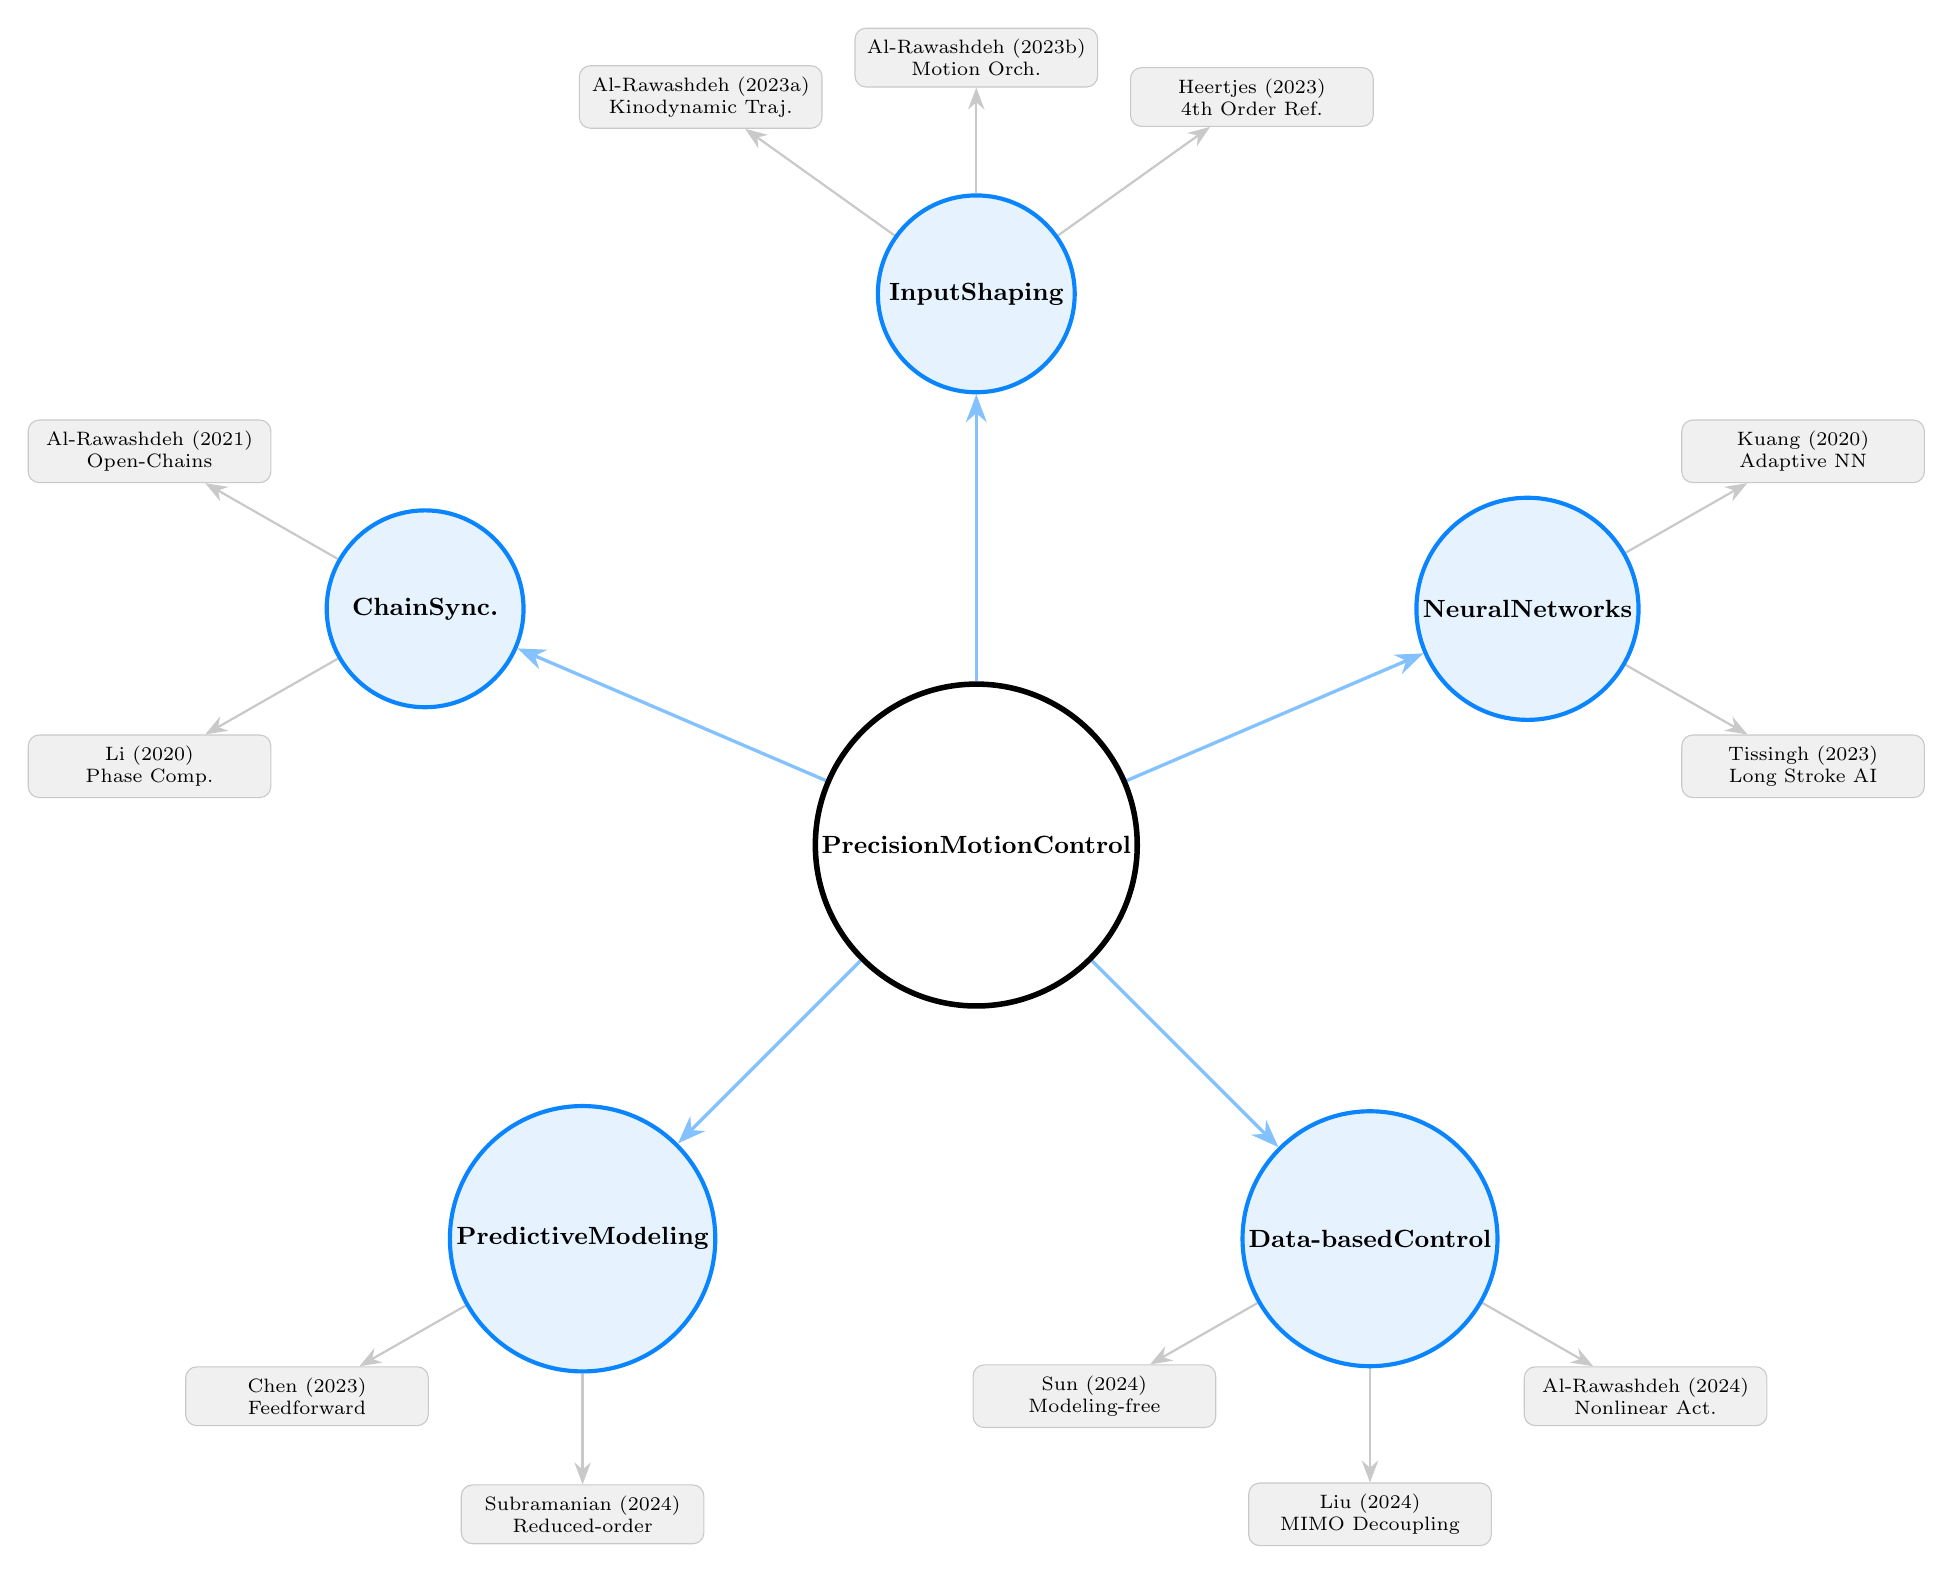
\begin{tikzpicture}[
    node distance=2cm,
    hub/.style={circle, draw=hubCol, fill=hubCol!10, line width=1.5pt, font=\bfseries\small, text centered, minimum size=2.5cm, inner sep=2pt},
    paper/.style={rectangle, draw=edgeCol, fill=paperCol, rounded corners, font=\scriptsize, text centered, inner sep=4pt, text width=2.8cm},
    edge/.style={->, >={Stealth[scale=1.2]}, line width=0.8pt, draw=edgeCol},
    background/.style={draw=none, fill=none}
]

% =====================================================================
% CENTRAL HUB: RESEARCH TOPIC
% =====================================================================
\node[hub, fill=white, draw=black, line width=2pt, minimum size=3cm] (CENTER) at (0,0) {Precision\\Motion\\Control};

% =====================================================================
% CATEGORY HUBS (PRISMA)
% =====================================================================

% 1. Input Shaping (Top)
\node[hub] (ISH) at (0, 7) {Input\\Shaping};
\node[paper] (p1) at (-3.5, 9.5) {Al-Rawashdeh (2023a)\\Kinodynamic Traj.};
\node[paper] (p2) at (0, 10) {Al-Rawashdeh (2023b)\\Motion Orch.};
\node[paper] (p3) at (3.5, 9.5) {Heertjes (2023)\\4th Order Ref.};

% 2. AI & Neural Networks (Right)
\node[hub] (AI) at (7, 3) {Neural\\Networks};
\node[paper] (p4) at (10.5, 5) {Kuang (2020)\\Adaptive NN};
\node[paper] (p5) at (10.5, 1) {Tissingh (2023)\\Long Stroke AI};

% 3. Data-based Control (Bottom Right)
\node[hub] (DATA) at (5, -5) {Data-based\\Control};
\node[paper] (p6) at (8.5, -7) {Al-Rawashdeh (2024)\\Nonlinear Act.};
\node[paper] (p7) at (5, -8.5) {Liu (2024)\\MIMO Decoupling};
\node[paper] (p8) at (1.5, -7) {Sun (2024)\\Modeling-free};

% 4. Predictive Modeling (Bottom Left)
\node[hub] (PRED) at (-5, -5) {Predictive\\Modeling};
\node[paper] (p9) at (-8.5, -7) {Chen (2023)\\Feedforward};
\node[paper] (p10) at (-5, -8.5) {Subramanian (2024)\\Reduced-order};

% 5. Chain Synchronization (Left)
\node[hub] (SYNC) at (-7, 3) {Chain\\Sync.};
\node[paper] (p11) at (-10.5, 5) {Al-Rawashdeh (2021)\\Open-Chains};
\node[paper] (p12) at (-10.5, 1) {Li (2020)\\Phase Comp.};

% 6. Foundations (Backplane)
% \node[hub, fill=orange!5, draw=orange!40] (FOUND) at (0, -2.5) {Foundations};

% =====================================================================
% EDGES
% =====================================================================
\begin{scope}[on background layer]
    % Center to Categories
    \foreach \h in {ISH, AI, DATA, PRED, SYNC}
        \draw[edge, line width=1.2pt, draw=hubCol!50] (CENTER) -- (\h);
    
    % Category Hubs to Papers
    \draw[edge] (ISH) -- (p1); \draw[edge] (ISH) -- (p2); \draw[edge] (ISH) -- (p3);
    \draw[edge] (AI) -- (p4); \draw[edge] (AI) -- (p5);
    \draw[edge] (DATA) -- (p6); \draw[edge] (DATA) -- (p7); \draw[edge] (DATA) -- (p8);
    \draw[edge] (PRED) -- (p9); \draw[edge] (PRED) -- (p10);
    \draw[edge] (SYNC) -- (p11); \draw[edge] (SYNC) -- (p12);
\end{scope}

\end{tikzpicture}
\end{document}
